\section{AJ-RNN}
``Adversarial Joint-Learning Recurrent Neural Network for Incomplete Time Series Classification" \cite{ajrnn} is a research paper that proposes a novel approach for classification of incomplete time series data.
The authors begin by highlighting the challenges of working with incomplete time series data, particularly the difficulty of extracting features and the need to deal with missing values.

To address these challenges, the authors propose an adversarial joint-learning recurrent neural network (AJ-RNN) that uses a recurrent neural network (RNN) to capture the temporal dependencies in the time series data, and an adversarial learning approach to impute the missing values.

The AJ-RNN is trained using a joint optimization framework that alternates between training the RNN for classification and the imputation network to fill in the missing values.
The adversarial component of the imputation network is used to ensure that the imputed values are as close as possible to the true values.

The authors evaluate the performance of the AJ-RNN on several real-world datasets and demonstrate that it outperforms several existing state-of-the-art approaches for time series classification.

\subsection{Adverarial learning}

% TODO review
Generative Adversarial Networks (GANs) have become popular in deep learning due to their potential for generating data according to the distribution of a real dataset \cite{goodfellow2014generative, ledig2017photo}.

The adversarial approach leads to better generation results than previous approaches [24], [25]. 
GANs have also been used to impute missing data in time series prediction with some success [26], [27], [28]. 
However, the question of how to employ adversarial learning in the domain of incomplete time series classification (ITSC) has not been previously explored.

In this paper we integrate adversarial training and joint (imputation and classification) learning in recurrent neural
networks (RNNs), and call our system Adversarial Joint learning RNN (AJ-RNN).

Our results demonstrate that this is an effective method to address the practical issue of incomplete time series classification in an end-to-end framework.
AJ-RNN is trained to approximate the value of the next input variable when it is revealed, and to fill it in with its prediction if it is missing. 
At the same time, AJ-RNN also learns to classify.
Hence AJ-RNN can directly perform classification with missing values.

\subsection{Data preparation}
- 

\subsection{Model}

% TODO rephrase

In this section, we present our model, the Adversarial Joint learning Recurrent Neural Network (AJ-RNN), to address the issue of time series classification with missing values.
The framework is shown in Figure \ref{fig:AJRNNrchitecture}. Here we describe how adversarial and joint learning strategies are integrated into an RNN.

We denote a time series $X = {x_1, x_2, ..., x_T }$ as a sequence vector of $T$ observations, where each observation $x_t \in R^d$.

Suppose a time series X has missing values
which can be indicated by a T-dimensional mask vector
$M = {m_1, m_2, ..., m_T}$, where $m_t \in {0, 1} \in R^d$, $m_t$ is $1$ if $x_t$ is revealed, and $0$ if $x_t$ is missing. 
Since we focus on incomplete time series classification, there is a target label $y^{(i)}$ for $i$-th time series $X^i$ given the time series data set $D$,
where $D = \{(X^i,M^i, y^i)\}^N_{i=1}$.

To avoid the traditional two-step approach, we regard imputation and classification as two tasks in multitask learning.
Specifically, the AJ-RNN is trained to approximate the value of the next input variable, using it as a target when it is revealed, while if the next value is missing, it will be filled in with the current prediction. 
At the same time, the AJ-RNN is trained to perform the classification task.

We solve the missing value problem by two processes: approximation and imputation. 
As seen in Fig. \ref{fig:AJRNNrchitecture}, two kinds of links enable AJ-RNN to directly model time series in the presence of missing values: dashed blue links (for approximation) and solid blue links (for imputation). 
We train $\hat{x_t}$ to approximate the next value $x_t$ when it is revealed using the last hidden states $h_{t-1}$ as follows:

\begin{equation}
  \hat{x_t} = W_{imp} h_{t-1} + b_z
\end{equation}

where $W_{imp} \in R^{n \times  m}$ is a learned regression matrix and $b_z$ is a bias term. 
Since $\hat{x_t}$ is trained to approximate the next value $x_t$, it can be used to impute it when missing. 
The input value $u_t$ is computed as:

\begin{equation}
  u_t = m_t \odot x_t + (1 - m_t) \odot \hat{x_t}
  \label{eq:AJRNNinput}
\end{equation}

where $m_t$ is the mask as defined above and $\odot$ is the elementwise product.

The RNN is trained using the completed input value $u_t$.
Formally, the update equation of the RNN is:

\begin{equation}
  h_t = F_{RNN} (h_{t-1}, u_t; W)
\end{equation}

Where $h_t$ represents the hidden unit vector at time $t$, $W$ encapsulates the input-to-hidden and hidden-to-hidden parameters, and $F_{RNN}$ represents the update function of the particular RNN variant.

Finally, the last hidden state of the RNN, $h_T$ , is fed into the classifier to obtain the probability distribution over each category label using a softmax:
\begin{equation}
  P(\hat{y_j}|h_T ) = \frac{exp(W^T_j  h_T )}{\sum_{l=1}^K exp(W^T_j  h_T )}
  \label{eq:AJRNNsoftmax}
\end{equation}

where $K$ is the number of class labels and $\{W_l\}^K_{l=1}$ are the class-specific weights of the softmax layer.
The classifier can use more complicated networks depending on the task.
We use this simple classifier because our main goal is to demonstrate mitigation of the exploding bias problem and report on the results achieved.
% For fairness, we use this approach for all methods, ours and the methods we implemented for comparison.

There are two tasks during the joint learning process, namely, imputation and classification. 
Let the superscript $i$ denote the $i$-th sample of the time series data set $D$.
For the imputation task, we can obtain the imputation sequence vector $\hat{X^i} = \{ \hat{x}^i_2, ..., \hat{x}^i_T \}$ 
of the $i$-th time series sample which can be divided into two parts, approximation values
(orange units in Fig. \ref{fig:AJRNNrchitecture}) and imputation ones (purple units
in Fig. \ref{fig:AJRNNrchitecture}). 
The imputation loss of all time series samples is calculated on the approximation values as follows:

\begin{equation}
  \mathcal{L}_{imp}(X, \hat{X}, M) = \frac{1}{N} \sum_{i=1}^N \lVert (X^i_{2:T} - \hat{X}^i) \odot M^i_{2:T} \rVert_2^2
  \label{eq:AJRNNimploss}
\end{equation}

where $N$ is the number of samples in the data set.
Equation (\ref{eq:AJRNNimploss}) is the mean squared error loss between the approximation and the revealed values.
$ M^i_{2:T}$ masks off the imputation values from the imputation loss since there is no ground truth for the missing values.

For the classification task, we obtain the predicted probability distribution $\hat{y}^i$ of $i$-th time series sample given by
Equation (\ref{eq:AJRNNsoftmax}), the loss of all samples of a time series can be calculated as follows:

\begin{equation}
  \mathcal{L}_{cls}(y, \hat{y}) = - \frac{1}{N} \sum_{i=1}^N \sum_{j=1}^K 1\{ y^i = j\} \log\hat{y}^i 
  \label{eq:AJRNNclsloss}
\end{equation}

where $K$ is the number of class labels. Equation (\ref{eq:AJRNNclsloss}) is the softmax cross entropy loss of the predicted label and the true label.

This end-to-end framework inevitably suffers from the negative impact (error propagation from imputation to classification) of missing values because the imputed values will contain some amount of error simply due to the fact that they are predictions.
This error can be quickly amplified as it is fed into the RNN, resulting in the exploding bias problem.

Here, we introduce a discriminator $D$ to reduce the negative impact of missing values. 
The discriminator $D$ distinguishes whether each value in the completed vector is real or imputed, rather than identifying the entire completed vector. 
In this way, the discriminator $D$ can provide direct supervision to the imputed values.

Specifically, for the $i$-th time series training sample, there is a completed sequence vector $U^i = \{u^i_2 , ..., u^i_T\}$
given by Equation (\ref{eq:AJRNNinput}) and its corresponding mask vector $M^i_{2:T} = \{m^i_2, ..., m^i_T \}$.

In $U^i$, some are real values, while the rest are imputed.
We know which are which by the mask vector $M^i$ . We can take advantage of this knowledge to provide a supervision signal for the imputation network.

The adversarial learning strategy is defined as a twoplayer minimax game.
We alternately update the parameters of discriminator $D$ and the parameters of the AJ-RNN.
First, $D$ receives the completed sequence vector as input and is trained to distinguish which values in the completed sequence vector are revealed and which are imputed. 
The discriminator loss can be defined as follows:

\begin{align}
  \mathcal{L}_{D}(U, M) & = - [E \log(D(X_{real})) + E \log(1 - D(\hat{X}_{imp}))] \label{eq:AJRNNdloss} \\ 
                        & = - \frac{1}{N} \sum_{i=1}^N \left[ M^i_{2:T} \odot \log(D(U^i)) + (1 - M^i_{2:T}) \odot \log(1-D(U^i)) \right]
\end{align}

where $D(\cdot)$ denotes the estimated mask probability $\hat{P}$ of the discriminator. 
In Equation (\ref{eq:AJRNNdloss}), the first term is the log output of the discriminator on real values, and the discriminator tries to maximize this to 1.
The second term isthe loss for imputed values.
Hence the discriminator tries to minimize its output for imputed values.

The discriminator is composed of 3 fully connected layers to take advantage of global contextual information (since it takes a sequence as input), where the number of units in the hidden layers are set to $T$ (i.e., the length of the sample), $T/2$, and $T$, respectively.
We use tanh as the activation function of each layer except for the output layer where we use the sigmoid activation function to get the estimated real/fake probability.

The RNN is thus supervised to make the distribution of predicted values is closer to the revealed ones by fooling the discriminator $D$. 
The adversarial loss of the RNN can be defined as follows:

\begin{equation}
  \mathcal{L}_{adv}(U, M) = \frac{1}{N} \sum_{i=1}^N  (1 - M^i_{2:T}) \odot \log(1 - D(U^i))
  \label{eq:AJRNNadvloss}
\end{equation}

Hence the AJ-RNN tries to maximize the discriminator output for imputed values.
This provides a supervisory signal for each imputed value in the completed sequence vector, which can reduce the bias introduced by the imputation operation and thus alleviate the exploding bias problem.
Note that we can also feed the whole imputation vector $\hat{X}^i$ into the discriminator, providing supervision for both the approximated and imputed values. 
In our experiments, we found that the results obtained by these two methods are similar. 
Hence, considering computational efficiency, we adopted Equation (\ref{eq:AJRNNadvloss}) as the adversarial loss.

Finally, the overall training loss of AJ-RNN is defined as follows:

\begin{equation}
  \mathcal{L}_{AJ-RNN} = \mathcal{L}_{cls} + \mathcal{L}_{imp} + \lambda_d \mathcal{L}_{adv}
  \label{eq:AJRNNloss}
\end{equation}

where $\lambda_d$ is hyper-parameter. This forms an end-to-end
training framework for incomplete time series classification.

AJ-RNN combines the merits of joint learning and adversarial learning.
The discriminator $D$ is trained with the revealed values and the mask vector effectively provides supervision on each imputed value. 
Therefore, the negative impact of missing values on AJ-RNN is reduced.

\begin{figure}[ht]
  \centering
  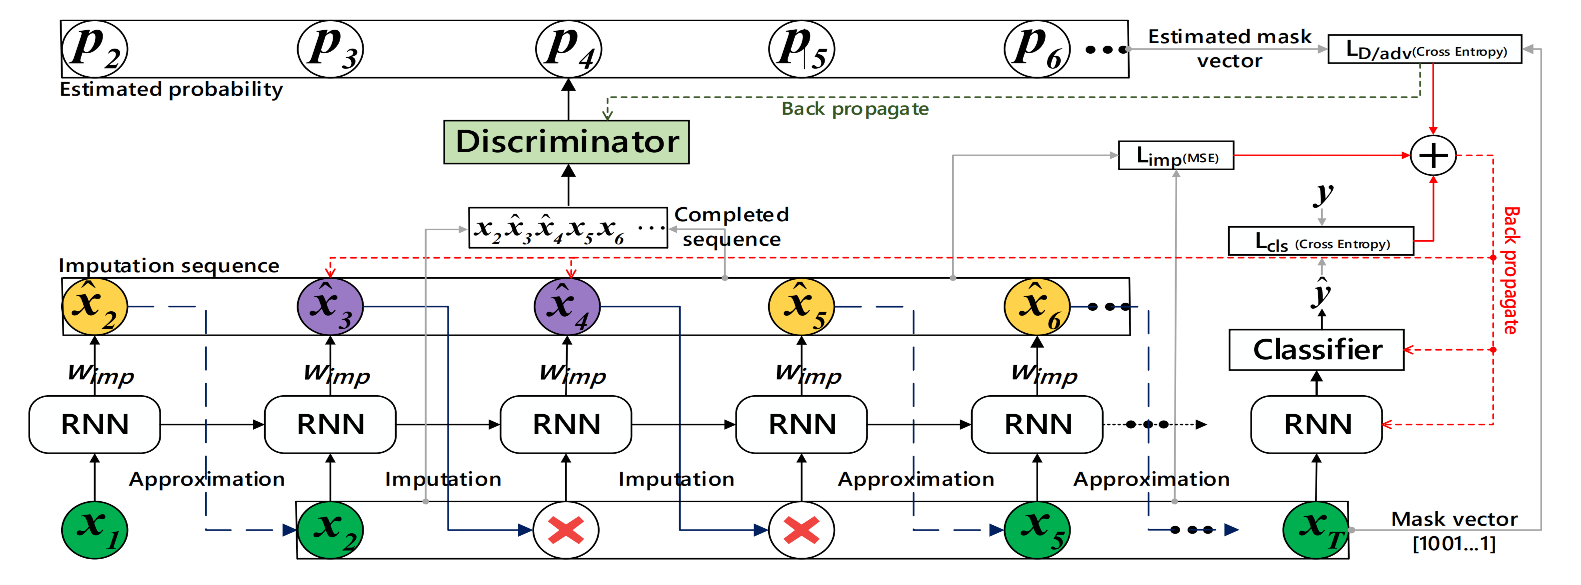
\includegraphics[width=1\textwidth]{ajrnn}
  \caption{The proposed AJ-RNN framework. We use green units to denote revealed inputs, yellow for the output of approximated values, purple for
  the imputed values and a red “X” for missing inputs. Dashed links are for approximation training and solid ones are for imputation. The discriminator
  receives a completed vector composed of revealed and imputed values as input, which provides a one-to-one supervisory signal for imputed values
  $\hat{x_3}$ and $\hat{x_4}$. \cite{ajrnn}}
  \label{fig:AJRNNrchitecture}
\end{figure}

\subsection{Experimental results}

% TODO review
The source code for the AJ-RNN model proveded by the authors is written in Python 2.7 and Tensorflow 1.0.
To enhance code readability and facilitate experimentation with different configurations, we have re-implemented the AJ-RNN model in Tensorflow 2.0 in a modularized fashion.
The implementation was carefully validated to ensure that the accuracy achieved by the model was consistent with the results reported in the paper using the same datasets. 

Additionally, the implementation was extended to support multivariate time series data to better fit our needs.

%- implemented in tensoflow 2.0 (modularized)\\
%-- made sure that acucracy was the same as in the paper\\
%-- added support for multivariate time series\\
- experimented with different configurations 

\begin{paragraph}{Cell type}
learning rate = 0.001, batch size = 256, G-epochs = 1

\begin{table}[!htbp]
  \centering
  \begin{tabular}{cccr} 
      Cell type & Cell size & Dropout & Overall Accuracy\\[0.2cm] 
      \hline \\[-0.2cm] 
      GRU   &   64  & 0.2 &  $84.10 \pm 3.72$\\
      GRU   &   64  & 0.4 &  $81.75 \pm 4.18$\\
      GRU   &   64  & 0.6 &  $79.70 \pm 4.92$\\
      GRU   &   64  & 0.8 &  $82.78 \pm 4.26$\\[0.05cm] \hline \\[-0.25cm]
      GRU   &   128 & 0.2 &  $78.58 \pm 4.17$\\
      GRU   &   128 & 0.4 &  $80.84 \pm 0.00$\\
      GRU   &   128 & 0.6 &  $70.07 \pm 9.58$\\
      GRU   &   128 & 0.8 &  $81.03 \pm 4.66$\\[0.05cm] \hline \\[-0.25cm]
      GRU   &   256 & 0.2 &  $80.49 \pm 8.77$\\
      GRU   &   256 & 0.4 &  $75.25 \pm 1.88$\\
      GRU   &   256 & 0.6 &  $75.97 \pm 1.43$\\
      GRU   &   256 & 0.8 &  $77.34 \pm 1.74$\\[0.05cm] \hline \\[-0.25cm]
      LSTM  &   64  & 0.2 &  $79.41 \pm 1.76$\\
      LSTM  &   64  & 0.4 &  $84.92 \pm 3.69$\\
      LSTM  &   64  & 0.6 &  $81.16 \pm 4.99$\\
      LSTM  &   64  & 0.8 &  $0.00 \pm 0.00$\\[0.05cm] \hline \\[-0.25cm]
      LSTM  &   128 & 0.2 &  $84.89 \pm 3.00$\\
      LSTM  &   128 & 0.4 &  $85.08 \pm 0.35$\\
      LSTM  &   128 & 0.6 &  $83.24 \pm 4.29$\\
      LSTM  &   128 & 0.8 &  $82.39 \pm 1.99$\\[0.05cm] \hline \\[-0.25cm]
      LSTM  &   256 & 0.2 &  $74.18 \pm 3.44$\\
      LSTM  &   256 & 0.4 &  $67.15 \pm 15.02$\\
      LSTM  &   256 & 0.6 &  $71.36 \pm 22.56$\\
      LSTM  &   256 & 0.8 &  $85.37 \pm 2.37$\\ 
      
  \end{tabular}
  \caption{Overall accuracy with different configurations for Cell type, Cell size and Dropout}
  \label{tab:AJRNNCellTypeResults}
\end{table}

\end{paragraph}

\begin{table}[!htbp]
  \centering
  \begin{tabular}{cccr} 
      Batch size & Learnig rate & Dropout & Overall Accuracy\\[0.2cm] 
      \hline \\[-0.2cm]
      256 &   1e-03 &   0.0 & $86.13 \pm 0.00$\\
      256 &   1e-03 &   0.2 & $78.58 \pm 4.17$\\
      256 &   1e-03 &   0.4 & $81.05 \pm 4.39$\\
      256 &   1e-03 &   0.6 & $73.03 \pm 9.81$\\
      256 &   1e-03 &   0.8 & $81.03 \pm 4.66$\\[0.05cm] \hline \\[-0.25cm]

      256 &   1e-04 &   0.4 & $80.00 \pm 2.91$\\
      256 &   1e-04 &   0.6 & $85.46 \pm 2.01$\\
      256 &   1e-04 &   0.8 & $83.88 \pm 4.33$\\[0.05cm] \hline \\[-0.25cm]

      32  &   1e-03 &   0.2 & $32.45 \pm 4.42$\\
      32  &   1e-03 &   0.6 & $28.21 \pm 6.00$\\
      32  &   1e-03 &   0.8 & $23.07 \pm 1.05$\\
      32  &   1e-04 &   0.0 & $30.26 \pm 0.00$\\[0.05cm] \hline \\[-0.25cm]

      32  &   1e-04 &   0.2 & $39.49 \pm 5.91$\\
      32  &   1e-04 &   0.4 & $28.93 \pm 0.00$\\
      32  &   1e-04 &   0.6 & $25.64 \pm 0.00$\\
      32  &   1e-04 &   0.8 & $32.97 \pm 0.00$\\[0.05cm] \hline \\[-0.25cm]

      32  &   1e-05 &   0.8 & $67.12 \pm 0.00$\\[0.05cm] \hline \\[-0.25cm]
      32  &   1e-08 &   0.0 & $73.32 \pm 2.83$
  \end{tabular}
  \caption{Overall accuracy with different configurations for Batch size, Learning rate and Dropout}
  \label{tab:AJRNNBatchSizeResults}
\end{table}


- learnig rate\\
- batch size \\
- G-epochs

\pagebreak
\subsection{Light AJ-RNN}
- model overview\\
- baseline

\begin{table}[!htbp]
  \centering
  \begin{tabular}{cccr} 
      Batch size & Learnig rate & Dropout & Overall Accuracy\\[0.2cm] 
      \hline \\[-0.2cm]
      256 & 0.0 & 1e-03 & $75.14 \pm 6.85$\\
      256 & 0.5 & 1e-03 & $78.48 \pm 0.00$\\[0.05cm] \hline \\[-0.25cm]

      256 & 0.0 & 1e-04 & $87.25 \pm 1.20$\\
      256 & 0.5 & 1e-04 & $82.60 \pm 2.17$\\
      256 & 0.8 & 1e-04 & $87.29 \pm 1.08$\\[0.05cm] \hline \\[-0.25cm]

      256 & 0.0 & 1e-05 & $83.29 \pm 2.85$\\
      256 & 0.0 & 1e-06 & $85.59 \pm 0.00$\\[0.05cm] \hline \\[-0.25cm]

      256 & 0.0 & 1e-07 & $81.72 \pm 3.32$\\
      256 & 0.5 & 1e-07 & $81.76 \pm 3.21$\\[0.05cm] \hline \\[-0.25cm]

      32  & 0.5 & 1e-03 & $30.85 \pm 0.00$\\[0.05cm] \hline \\[-0.25cm]

      32  & 0.0 & 1e-04 & $33.55 \pm 2.42$\\
      32  & 0.5 & 1e-04 & $32.33 \pm 1.33$\\[0.05cm] \hline \\[-0.25cm]

      32  & 0.0 & 1e-05 & $44.23 \pm 12.02$\\[0.05cm] \hline \\[-0.25cm]
      32  & 0.0 & 1e-06 & $54.32 \pm 13.73$\\[0.05cm] \hline \\[-0.25cm]
      32  & 0.0 & 1e-07 & $52.98 \pm 15.22$\\[0.05cm] \hline \\[-0.25cm]
      32  & 0.0 & 1e-08 & $55.80 \pm 11.27$\\
      32  & 0.5 & 1e-08 & $52.32 \pm 11.36$\\
  \end{tabular}
  \caption{Overall accuracy with different configurations for Batch size, Learning rate and Dropout}
  \label{tab:AJRNNBatchSizeResults}
\end{table}
